\chapter{Transmission Handler}
\label{chap_transmission}

Transmission Handler berfungsi menangani pengiriman dan penerimaan pesan APDU Command dan Response dari dan ke terminal. Pengiriman dan Penerimaan byte data pesan secara aktual dilakukan menggunakan fungsi HAL IO yang sesuai. Melalui antarmuka yang disediakan Transmission Handler, modul-modul pintarOS lainnya (terutama Command Handlers) tidak perlu mengetahui protokol yang digunakan pada proses pengiriman/penerimaan pesan APDU.

Tabel \ref{tabel-func-transmission} menampilkan fungsi-fungsi yang terdapat pada modul Transmission beserta kegunaannya.

\begin{table}[h]
  \centering
  \begin{tabular}{|m{5cm}|m{8cm}|}
    \hline
    \bf{Nama Fungsi} & \bf{Kegunaan} \\
    \hline
    Get Byte & Menerima 1 byte data menggunakan protokol yang dipilih \\
    \hline
    Send Byte & Mengirim 1 byte data menggunakan protokol yang dipilih \\
    \hline
    Get Header & Menerima bagian header dari Command APDU \\
    \hline
    Get Data & Menerima bagian data dari Command APDU \\
    \hline
    Send Data & Mengirimkan bagian data dari Response APDU \\
    \hline
    Send SW & Mengirimkan bagian SW1 dan SW2 dari Response APDU \\
    \hline
  \end{tabular}
  \caption{Daftar antarmuka fungsi yang disediakan Transmission Handler}
  \label{tabel-func-transmission}
\end{table}


\section{Get Byte}
\label{sec_getbyte}

Berfungsi menerima 1 byte data dari IO menggunakan protokol komunikasi yang dipilih. Gambar \ref{fig-dfd-getbyte} menampilkan DFD dari fungsi Transmission Get Byte (RxByte). Diagram alir fungsi kemudian ditampilkan pada Gambar \ref{fig-flow-getbyte}. 

\begin{figure}[!h]
\centering
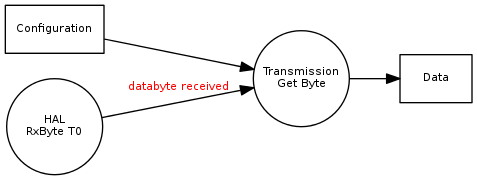
\includegraphics[width=0.75\textwidth]{image/transmission/dfd_getbyte.png}
\caption{DFD Transmission GetByte}
\label{fig-dfd-getbyte}
\end{figure}

\begin{figure}[!h]
\centering
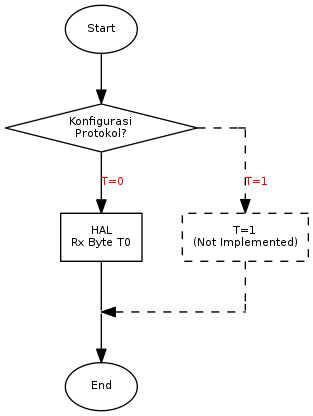
\includegraphics[height=0.4\textheight]{image/transmission/flow_getbyte.png}
\caption{Flowchart Transmission Get Byte}
\label{fig-flow-Get Byte}
\end{figure}

\subsection {Pengujian}

\begin{table}[h]
  \centering
  \begin{tabular}{ | c || c | }
    \hline
    \bf{Input}  & \bf{Output} \\
    \hline
    \bf{Databyte (from terminal)} & \bf{Return Value}\\
    \hline
    0x00 & = 0x00 \\
    0x01 & = 0x01 \\
    \hline
    \multicolumn{2}{ |c| }{...} \\
    \multicolumn{2}{ |c| }{...} \\
    \hline
    0xff & = 0xff \\
    \hline
  \end{tabular}
  \caption{Test Vector Fungsi Transmission GetByte}
  \label{tabel-test-getbyte}
\end{table}

Tabel \ref{tabel-test-getbyte} menampilkan Test Vector yang digunakan untuk menguji fungsi Transmission Get Byte.

\subsection {Implementasi}

Tabel \ref{tabel-getbyte} menampilkan purwarupa dari implementasi fungsi Transmission Get Byte. 

\begin{table}[!h]
  \centering
  \begin{tabular}{p{2cm} p{8cm}}
    \hline\\
    {\bf Name} & Transmission\_GetByte\\
    \hline\\
    {\bf Input} & 
    \\
    \hline\\
    {\bf Output} & Data yang diterima (1 byte)
    \\
    \hline
  \end{tabular}
  \caption{Prototype Fungsi Transmission Get Byte}
  \label{tabel-getbyte}
\end{table}

Listing \ref{list-getbyte} menampilkan potongan program yang mengimplementasi fungsi Transmission Get Byte.

\begin{lstlisting}[caption={Listing Program Fungsi Transmisison Get Byte}, label={list-getbyte}]
uint8_t Transmission_GetByte()
{
  /* if (config.proto == 0) */
    return HAL_RxByteT0();
}
\end{lstlisting}


\section{Send Byte}
\label{sec_sendbyte}

Berfungsi mengirimkan 1 byte data menggunakan protokol komunikasi yang dipilih. Gambar \ref{fig-dfd-sendbyte} menampilkan DFD dari fungsi Transmission Send Byte (RxByte). Diagram alir fungsi kemudian ditampilkan pada Gambar \ref{fig-flow-sendbyte}. 

\begin{figure}[!h]
\centering
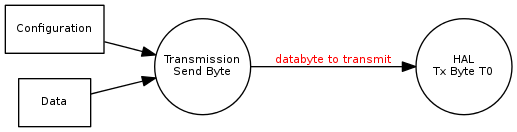
\includegraphics[width=0.75\textwidth]{image/transmission/dfd_sendbyte.png}
\caption{DFD Transmission Send Byte}
\label{fig-dfd-sendbyte}
\end{figure}

\begin{figure}[!h]
\centering
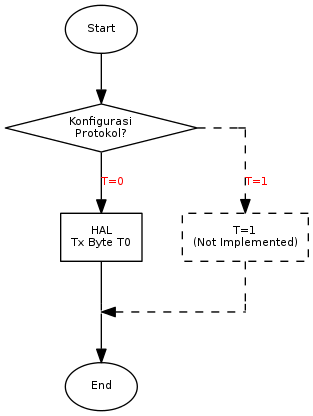
\includegraphics[height=0.4\textheight]{image/transmission/flow_sendbyte.png}
\caption{Flowchart Transmission Send byte}
\label{fig-flow-sendbyte}
\end{figure}

\subsection {Pengujian}

\begin{table}[h]
  \centering
  \begin{tabular}{ | c || c | }
    \hline
    \bf{Input}  & \bf{Output} \\
    \hline
    \bf{Data} & \bf{Databyte (to terminal)}\\
    \hline
    0x00 & = 0x00 \\
    0x01 & = 0x01 \\
    \hline
    \multicolumn{2}{ |c| }{...} \\
    \multicolumn{2}{ |c| }{...} \\
    \hline
    0xff & = 0xff \\
    \hline
  \end{tabular}
  \caption{Test Vector Fungsi Transmission SendByte}
  \label{tabel-test-sendbyte}
\end{table}

Tabel \ref{tabel-test-sendbyte} menampilkan Test Vector yang digunakan untuk menguji fungsi Transmission Send Byte.

\subsection {Implementasi}

Tabel \ref{tabel-sendbyte} menampilkan purwarupa dari implementasi fungsi Transmission Send Byte. 

\begin{table}[!h]
  \centering
  \begin{tabular}{p{2cm} p{8cm}}
    \hline\\
    {\bf Name} & Transmission\_SendByte\\
    \hline\\
    {\bf Input} & Data yang akan dikirimkan (1 byte)
    \\
    \hline\\
    {\bf Output} & -
    \\
    \hline
  \end{tabular}
  \caption{Prototype Fungsi Transmission Send Byte}
  \label{tabel-sendbyte}
\end{table}

Listing \ref{list-sendbyte} menampilkan potongan program yang mengimplementasi fungsi Transmission Send Byte.

\begin{lstlisting}[caption={Listing Program Fungsi Transmisison Send Byte}, label={list-sendbyte}]
void Transmission_SendByte(uint8_t databyte)
{
  /* if (config.protocol == 0) */
    HAL_TxByteT0(databyte);
}
\end{lstlisting}


\section{Get Header}
\label{sec_getheader}

Berfungsi menerima 5 byte pertama dari command APDU (header). Header ini kemudian disimpan pada variable array \emph{header} yang terdapat pada \emph{Command Handlers}. Gambar \ref{fig-dfd-getheader} menampilkan DFD dari fungsi Get Header. Diagram alir fungsi kemudian ditampilkan pada Gambar \ref{fig-flow-getheader}.

\begin{figure}[!h]
\centering
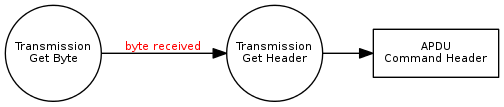
\includegraphics[width=0.75\textwidth]{image/transmission/dfd_getheader.png}
\caption{DFD Transmission Get Header}
\label{fig-dfd-getheader}
\end{figure}

\begin{figure}[!h]
\centering
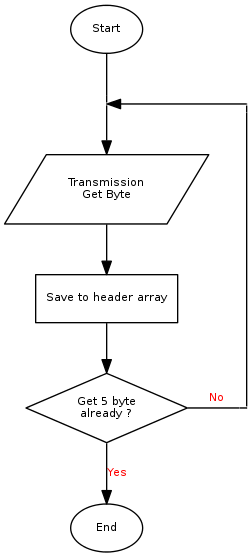
\includegraphics[height=0.5\textheight]{image/transmission/flow_getheader.png}
\caption{Flowchart Transmission Get Header}
\label{fig-flow-getheader}
\end{figure}

\subsection {Pengujian}

\begin{table}[h]
  \centering
  \begin{tabular}{ | c || c | }
    \hline
    \bf{Input}  & \bf{Output} \\
    \hline
    \bf{Databyte} & \bf{header}\\
    \hline
    [0x00,0x01,0x02,0x03,0x04,..,0x0f] & = [0x00,0x01,0x02,0x03,0x04] \\
    \hline
  \end{tabular}
  \caption{Test Vector Fungsi Transmission GetHeader}
  \label{tabel-test-getheader}
\end{table}

Tabel \ref{tabel-test-getheader} menampilkan Test Vector yang digunakan untuk menguji fungsi Transmission Get Header.


\subsection {Implementasi}

Tabel \ref{tabel-getheader} menampilkan purwarupa dari implementasi fungsi Transmission Get Header.

\begin{table}[!h]
  \centering
  \begin{tabular}{p{2cm} p{8cm}}
    \hline\\
    {\bf Name} & Transmission\_GetHeader\\
    \hline\\
    {\bf Input} & -
    \\
    \hline\\
    {\bf Output} & -
    \\
    \hline
  \end{tabular}
  \caption{Prototype Fungsi Transmission Get Header}
  \label{tabel-getheader}
\end{table}

Listing \ref{list-getheader} menampilkan potongan program yang mengimplementasi fungsi Get Header.

\begin{lstlisting}[caption={Listing Program Fungsi Get Header}, label={list-getheader}]
void Transmission_GetHeader()
{
  uint8_t i;

  for (i = 0; i < 5; ++i)
    {
      header[i] = Transmission_GetByte();
    }
}
\end{lstlisting}


\section{Get Data}
\label{sec_getdata}

Berfungsi menerima bagian data dari Command APDU, yang diperoleh dari dari IO, untuk digunakan oleh \emph{command handler}. Gambar \ref{fig-dfd-getdata} menampilkan DFD dari fungsi Get Data. Diagram alir fungsi kemudian ditampilkan pada Gambar \ref{fig-flow-getdata}.

\begin{figure}[!h]
\centering
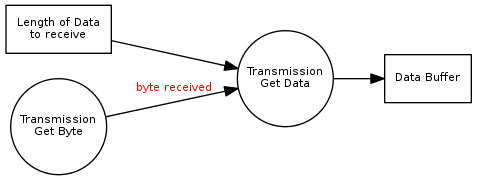
\includegraphics[width=0.75\textwidth]{image/transmission/dfd_getdata.png}
\caption{DFD Transmission Get Data}
\label{fig-dfd-getdata}
\end{figure}

\begin{figure}[!h]
\centering
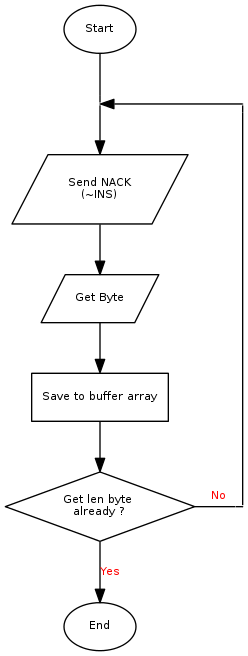
\includegraphics[height=0.5\textheight]{image/transmission/flow_getdata.png}
\caption{Flowchart Get Data}
\label{fig-flow-getdata}
\end{figure}

\subsection {Pengujian}

\begin{table}[h]
  \centering
  \begin{tabular}{ | c | c || c | }
    \hline
    \multicolumn{2}{ |c|| }{\bf{Input}}  & \bf{Output} \\
    \hline
    \bf{Databyte (from terminal)} & \bf{length} & \bf{output buffer} \\
    \hline
    {[0x00,0x01,0x02,0x03,0x04,..,0x0f]} & 1 & {[=0x00]} \\
    {[0x00,0x01,0x02,0x03,0x04,..,0x0f]} & 2 & {[=0x00,0x01]} \\
    {[0x00,0x01,0x02,0x03,0x04,..,0x0f]} & 3 & {[=0x00,0x01,0x02]} \\
    {[0x00,0x01,0x02,0x03,0x04,..,0x0f]} & 4 & {[=0x00,0x01,0x02,0x03]} \\
    {[0x00,0x01,0x02,0x03,0x04,..,0x0f]} & 5 & {[=0x00,0x01,0x02,0x03,0x04]} \\
    \hline
  \end{tabular}
  \caption{Test Vector Fungsi Transmission GetData}
  \label{tabel-test-getdata}
\end{table}

Tabel \ref{tabel-test-getdata} menampilkan Test Vector yang digunakan untuk menguji fungsi Transmission Get Data.

\subsection {Implementasi}

Tabel \ref{tabel-getdata} menampilkan purwarupa dari implementasi fungsi Transmission Get Data.

\begin{table}[!h]
  \centering
  \begin{tabular}{p{2cm} p{8cm}}
    \hline\\
    {\bf Name} & Transmission\_GetData\\
    \hline\\
    {\bf Input} & 
    \begin{itemize}[noitemsep,topsep=0pt,parsep=0pt,partopsep=0pt]
    \item Alamat buffer dimana data akan disimpan
    \item Panjang data yang akan diterima
    \end{itemize}
    \\
    \hline\\
    {\bf Output} & -
    \\
    \hline
  \end{tabular}
  \caption{Prototype Fungsi Get Data}
  \label{tabel-getdata}
\end{table}

Listing \ref{list-getdata} menampilkan potongan program yang mengimplementasi fungsi Get Data.

\begin{lstlisting}[caption={Listing program fungsi Get Data}, label={list-getdata}]
void Transmission_GetData(uint8_t * dst, uint8_t len)
{
  while ( len>0 )
    {
      Transmission_SendNACK();
      *(dst++) = Transmission_GetByte();
      len--;
    }
}
\end{lstlisting}

\section{Send Data}
\label{sec_senddata}

Berfungsi mengirimkan bagian data dari Response APDU. Digunakan oleh \emph{command handler}. Gambar \ref{fig-dfd-senddata} menampilkan DFD dari fungsi Get Header. Diagram alir fungsi kemudian ditampilkan pada Gambar \ref{fig-flow-senddata}.

\begin{figure}[!h]
\centering
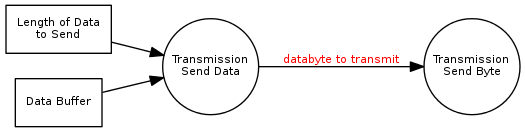
\includegraphics[width=0.75\textwidth]{image/transmission/dfd_senddata.png}
\caption{DFD Transmission Send Data}
\label{fig-dfd-senddata}
\end{figure}

\begin{figure}[!h]
\centering
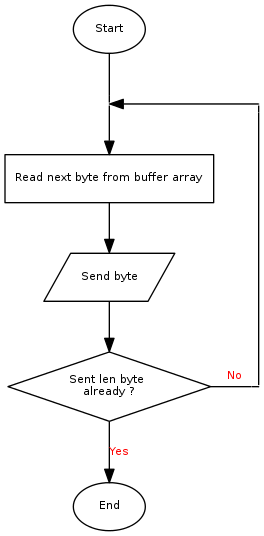
\includegraphics[height=0.5\textheight]{image/transmission/flow_senddata.png}
\caption{Flowchart Transmission Send Data}
\label{fig-flow-senddata}
\end{figure}

\subsection {Pengujian}

\begin{table}[h]
  \centering
  \begin{tabular}{ | c | c || c | }
    \hline
    \multicolumn{2}{ |c|| }{\bf{Input}}  & \bf{Output} \\
    \hline
    \bf{input buffer} & \bf{length} & \bf{databyte (to terminal)}\\
    \hline
    {[0x00,0x01,0x02,0x03,0x04,..,0x0f]} & 1 & = {[0x00]} \\
    {[0x00,0x01,0x02,0x03,0x04,..,0x0f]} & 2 & = {[0x00,0x01]} \\
    {[0x00,0x01,0x02,0x03,0x04,..,0x0f]} & 3 & = {[0x00,0x01,0x02]} \\
    {[0x00,0x01,0x02,0x03,0x04,..,0x0f]} & 4 & = {[0x00,0x01,0x02,0x03,]} \\
    {[0x00,0x01,0x02,0x03,0x04,..,0x0f]} & 5 & = {[0x00,0x01,0x02,0x03,0x04]} \\
    \hline
  \end{tabular}
  \caption{Test Vector Fungsi Transmission SendData}
  \label{tabel-test-senddata}
\end{table}

Tabel \ref{tabel-test-senddata} menampilkan Test Vector yang digunakan untuk menguji fungsi Transmission Send Data.



\subsection {Implementasi}

Tabel \ref{tabel-senddata} menampilkan purwarupa dari implementasi fungsi Transmission Send Data. 

\begin{table}[!h]
  \centering
  \begin{tabular}{p{2cm} p{8cm}}
    \hline\\
    {\bf Name} & Transmission\_SendData\\
    \hline\\
    {\bf Input} & 
    \begin{itemize}[noitemsep,topsep=0pt,parsep=0pt,partopsep=0pt]
    \item Alamat dari buffer data yang akan dikirim
    \item Panjang data yang akan dikirimkan
    \end{itemize}
    \\
    \hline\\
    {\bf Output} & -
    \\
    \hline
  \end{tabular}
  \caption{Prototype Fungsi Send Data}
  \label{tabel-senddata}
\end{table}

Listing \ref{list-senddata} menampilkan potongan program yang mengimplementasi fungsi Send Data.

\begin{lstlisting}[caption={Listing program fungsi Send Data}, label={list-senddata}]
void Transmission_SendData(uint8_t * src, uint8_t len)
{
  while ( len>0 )
    {
      Transmission_SendByte( *(src++) );
      len--;
    }
}
\end{lstlisting}

\section{Send SW}
\label{sec_sendsw}

Berfungsi mengirimkan Status Word dari Response APDU. Status Word yang akan dikirimkan diperoleh dari variable \emph{sw} yang telah di-set oleh \emph{Response\_SetSW}. Gambar \ref{fig-dfd-sendsw} menampilkan DFD dari fungsi Send SW. Diagram alir fungsi kemudian ditampilkan pada Gambar \ref{fig-flow-sendsw}.

\begin{figure}[!h]
\centering
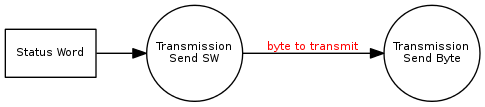
\includegraphics[width=0.75\textwidth]{image/transmission/dfd_sendsw.png}
\caption{DFD Transmission Send SW}
\label{fig-dfd-sendsw}
\end{figure}

\begin{figure}[!h]
\centering
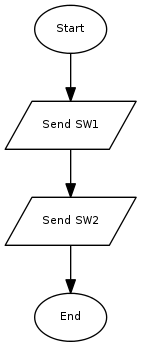
\includegraphics[height=0.3\textheight]{image/transmission/flow_sendsw.png}
\caption{Flowchart Send SW}
\label{fig-flow-sendsw}
\end{figure}

\subsection {Pengujian}

\begin{table}[h]
  \centering
  \begin{tabular}{ | c | c || c | }
    \hline
    {\bf{Input}}  & \bf{Output} \\
    \hline
    \bf{SW} & \bf{output buffer}\\
    \hline
    0x9000 & = [0x90,0x00] \\
    0x63C1 & = [0x63,0xC1] \\
    \hline
  \end{tabular}
  \caption{Test Vector Fungsi Transmission Send SW}
  \label{tabel-test-sendsw}
\end{table}

Tabel \ref{tabel-test-sendsw} menampilkan Test Vector yang digunakan untuk menguji fungsi Transmission Send SW.

\subsection {Implementasi}

Tabel \ref{tabel-sendsw} menampilkan purwarupa dari implementasi fungsi Transmission Send SW. 

\begin{table}[!h]
  \centering
  \begin{tabular}{p{2cm} p{8cm}}
    \hline\\
    {\bf Name} & Transmission\_SendSW\\
    \hline\\
    {\bf Input} & -
    \\
    \hline\\
    {\bf Output} & -
    \\
    \hline
  \end{tabular}
  \caption{Prototype Fungsi Transmission Send SW}
  \label{tabel-sendsw}
\end{table}

Listing \ref{list-sendsw} menampilkan potongan program yang mengimplementasi fungsi Transmission Send SW.

\begin{lstlisting}
void Transmission_SendSW()
{
  Transmission_SendByte( ( (uint8_t)(sw>>8) & 0xFF) );
  Transmission_SendByte( (uint8_t)(sw & 0xFF) );
}
\end{lstlisting}
\caption{Listing program fungsi Send SW}
\label{list-sendsw}
